\chapter{Introduction}
\label{chap:introduction}
\pagenumbering{arabic}% Arabic page numbers (and reset to 1)
In this chapter, the topic of this dissertation is first positioned in the research area and its objectives are developed. Following, a more specific definition of the topic will be given. Subsequently, the research objective and hypothesis will be presented.
\section{Background and Motivation}

Accidental pollutant spills in rivers can influence the water quality and the hydrodynamics of the flow over large portions of the channel. Therefore, the calculation of mass transport on rivers is an important aspect to determine the extension of the damage. The parameters that dictate the solute transport in streams and rivers are strongly related to geometric and hydrodynamic characteristics of the river (e.g., velocity distribution, channel width, flow depth, vortex shedding). Over large distances, the mass transport is mainly restricted to the length and thus it takes a 1-dimensional approach \cite{weitbrecht2004}. Although, the complexity of this solute transport must take into account different aspects of the river over its length, as rivers do not have a constant geometry over all its length. The accountability of the cross-section of the river leads to a 2-dimensional model. Despite the model now offer a variability range, there are aspects in natural and regulated rivers that introduce the third dimension due to rapid changes in the depth direction. Still, regions such as dead zones (DZ), that are regions separated from the main channel and have a net flux close to zero in the main stream direction which configures these structures as transient storage volumes. The formation of DZ can occur from any structure that creates an irregularity within the water body morphology, examples of structures are: groyne fields, lateral cavities, vanes, harbours and sidearms. The shared characteristic of these zones is its closeness, except for a single interface, the volume is completely dissociated from the main channel. This implies that the study of this interface is essential to understand all the exchange processes between the DZ and the main channel.

Normally placed in shallow waters, the transport inside the DZ is regarded as a two-dimensional motion, except for the interface between the unaltered channel (main channel) and the DZ where complex three-dimensional motion occurs \cite{xiang2020}. The typical path in the interface follows the order where the fluid penetrates the DZ near the bottom of the channel and exits primarily in the top layer of the flow, also it enters approximately via the downstream portion and exits in the upstream of the DZ \cite{weitbrecht2004,xiang2020}. This structure can be considered as a transient storage volume.

The transient storage of mass inside the DZ has been known to provide refuge to aquatic communities as they seek shelter in slower-moving flows in the surface stream or the hyporheic zone \cite{jackson2013}. According to the same author, the benefits of this storage extends to water quality improvement as the solutes residence times increases further increasing the interaction of nutrient-rich surface waters with biogeochemically-reactive sediments. For instance, \textcite{SchwartzKozerski2003} detected in their sample larger amounts of element contents with sedimentary origin than from geogenic sources, the increase in mass settled to the riverbed. These settled matter can favour vegetation growth (Figure \ref{fig:satelliteImage}). The drag created by the presence of vegetation changes the flow and consequently the mass exchange rates, which increases the uncertainty of volumes captured within the seasons.

\begin{figure}[!ht]
\centering
\begin{subfigure}{0.49\textwidth}
  \centering
  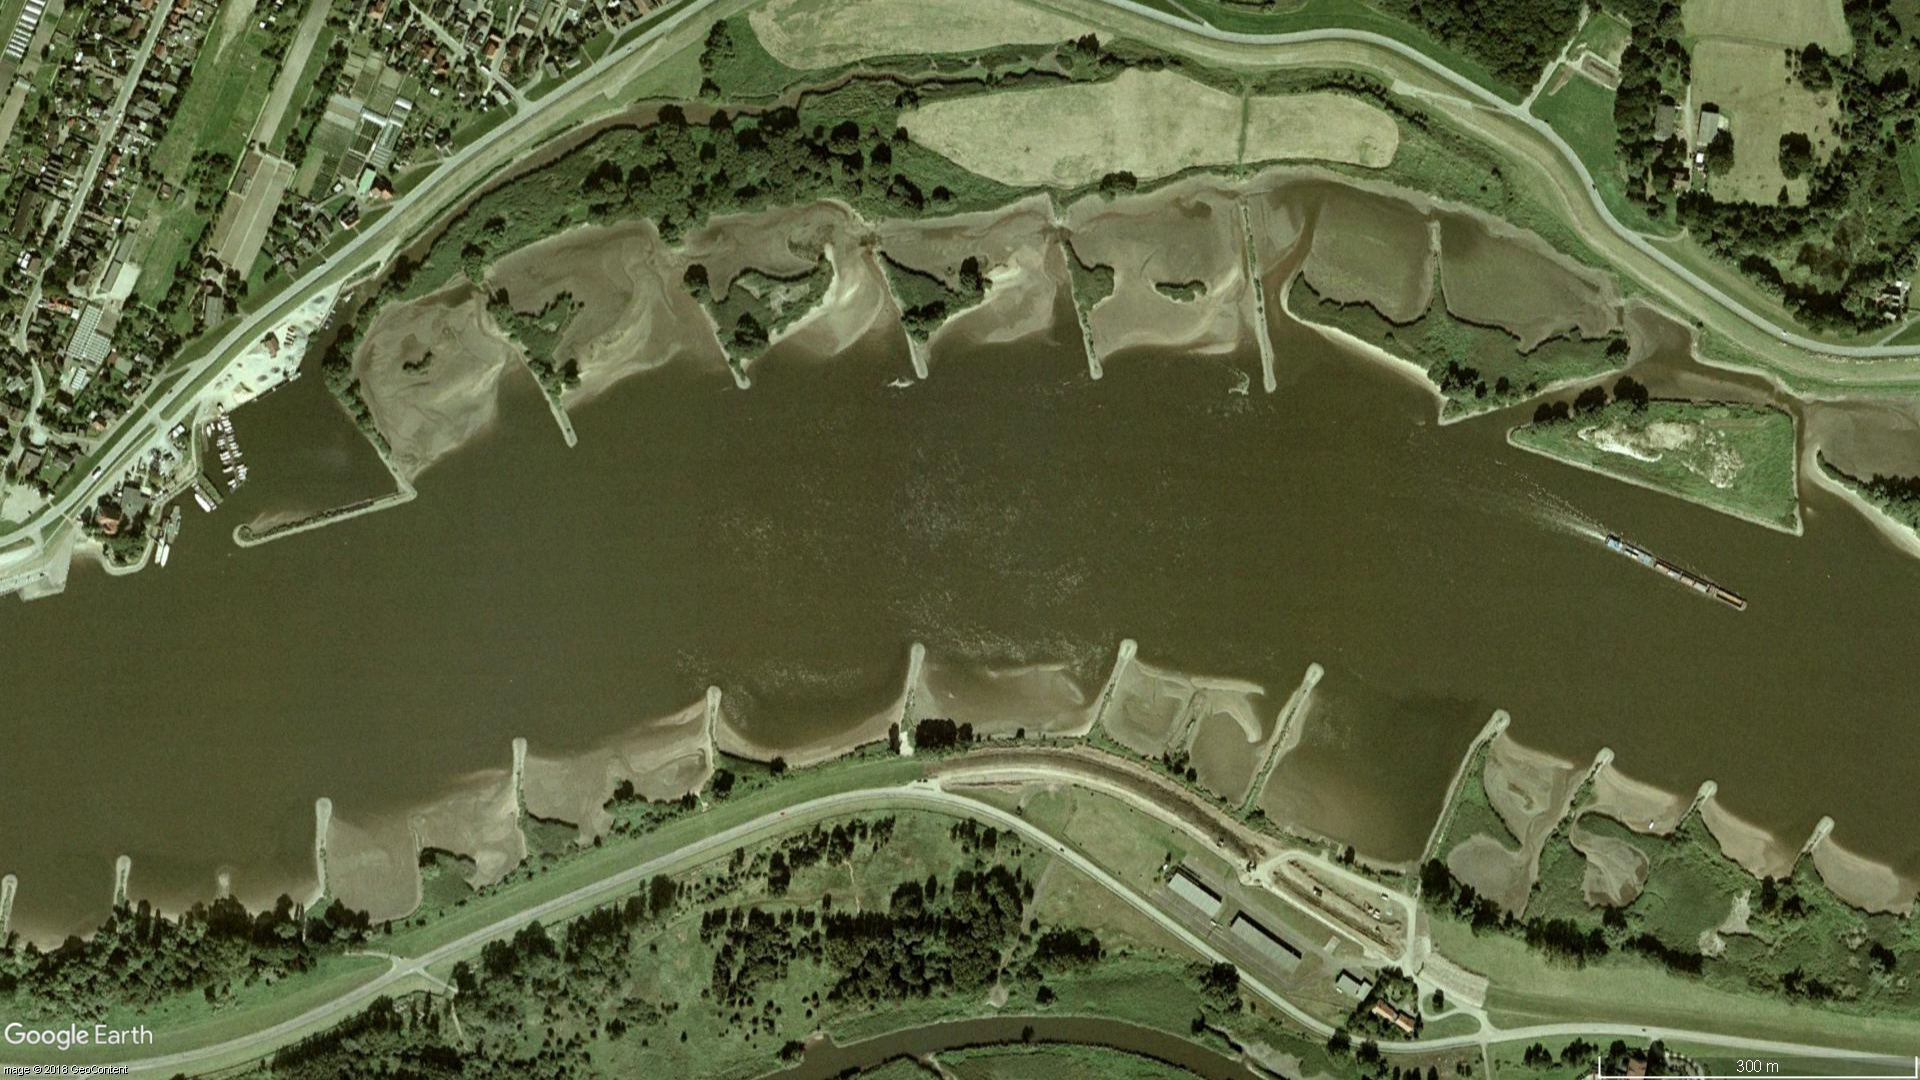
\includegraphics[width=0.9\linewidth]{../images/introduction/sat2000.jpg}
  \caption{2000}
  \label{fig:sat2000}
\end{subfigure}%
\begin{subfigure}{.49\textwidth}
  \centering
  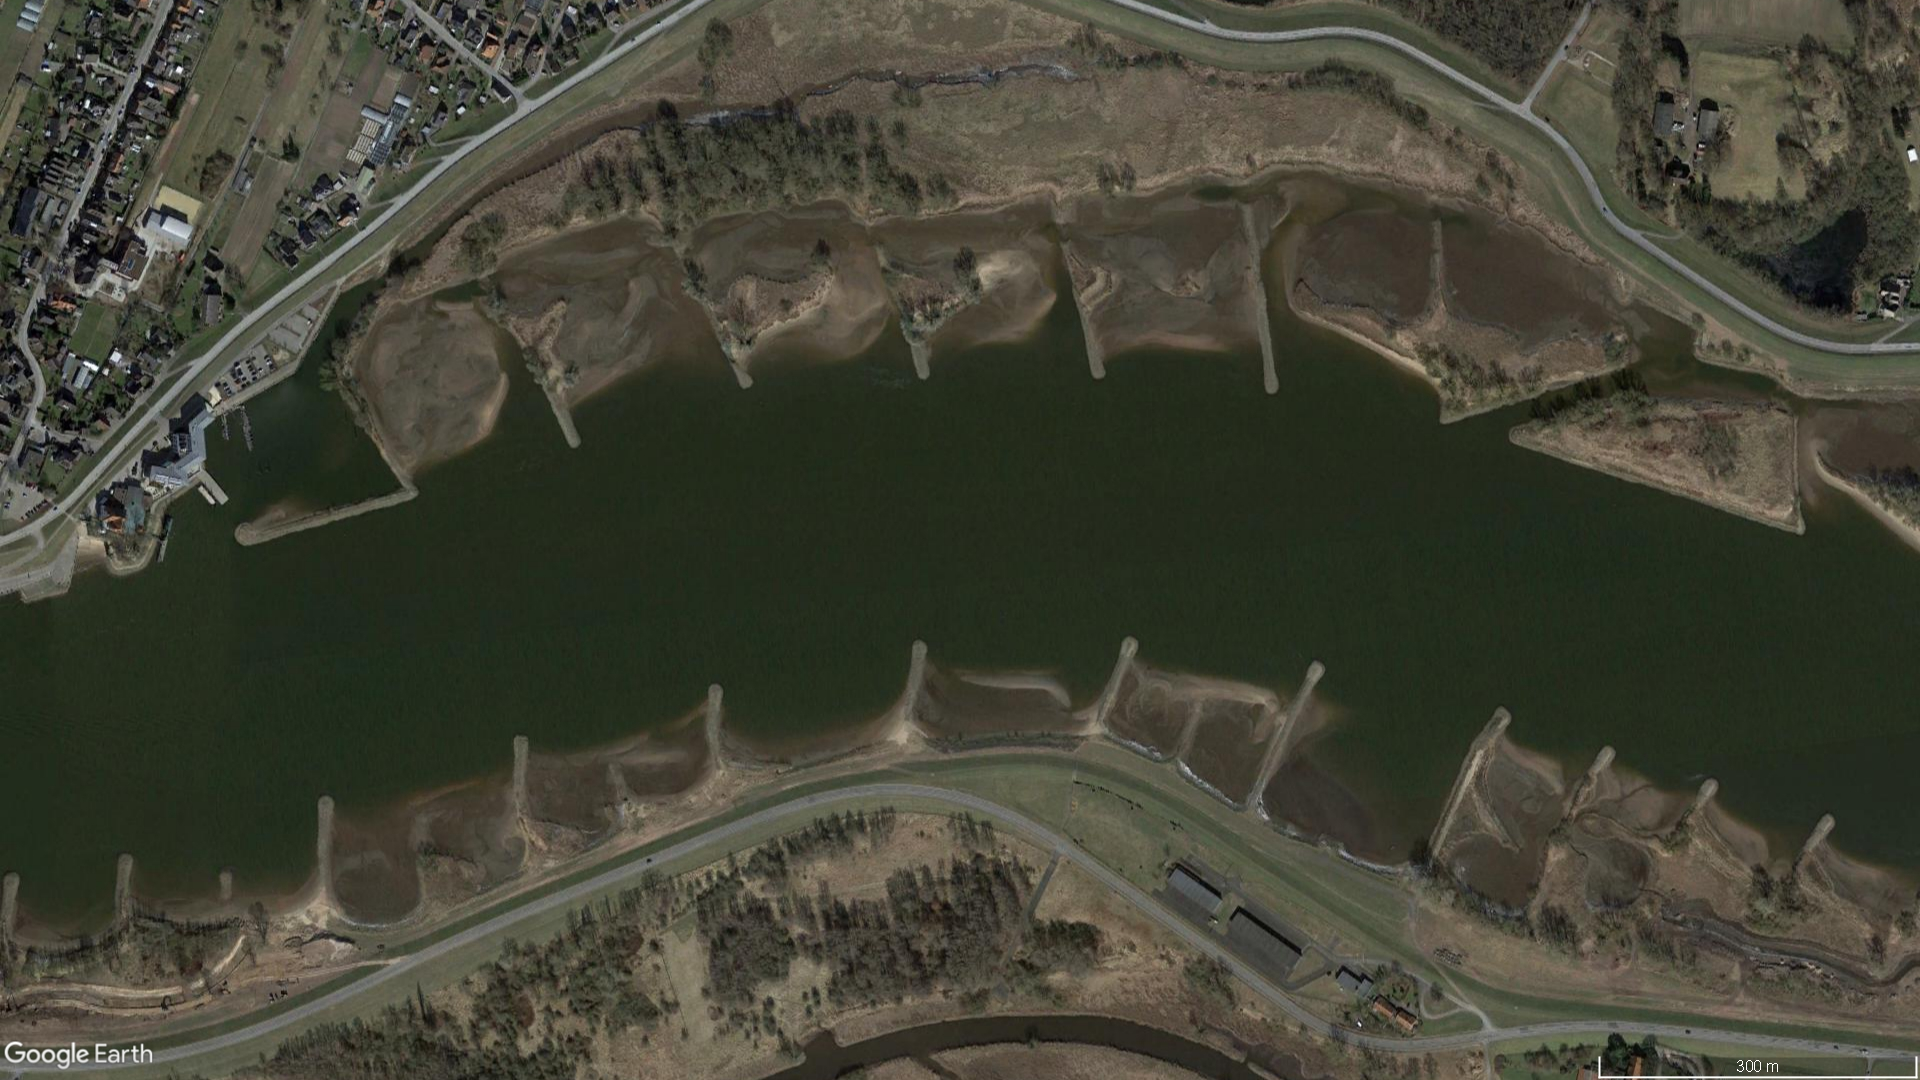
\includegraphics[width=0.9\linewidth]{../images/introduction/sat2018.jpg}
  \caption{2018}
  \label{fig:sat2018}
\end{subfigure}
\caption{Groyne Fields 53\degree23'54.32" N,  10\degree11'51.08" E, elevation 1.90 km. Terrain layer, viewed 29 August 2019. <http://www.google.com/earth/index.html>}
\label{fig:satelliteImage}
\end{figure}
\section{Hydrodynamics and Mass Exchange}
The DZ is created by transversal structures placed on the riverbank, these structures diverge the flow creating a rotational field. The importance of DZ is due (1) the enhancement in biodiversity \cite{ribi2014,harvey2016}, (2) the function as a macro-roughness at the river banks, mitigating erosion \cite{Juez2018} and (3) act as a transient storage zone \cite{jackson2013,drost2014,jackson2015}. The principal characteristic of the flow, in an emergent scenario, is the presence of gyres. These vortexes origin from the dissipation of moment that occurs in the interface layer between the DZ and the main channel. The shearing and flow separation at the leading edge form a mixing layer that extends until the downstream portion of the lateral cavity \cite{uijttewaal2005,jackson2013}. The shape and quantity of circulations inside the cavity are determined by a geometric aspect between the width (normal to the flow, \textit{W}) and length (parallel to the flow, \textit{L}) of the cavity. The aspect ratio \textit{W/L} divides the flow in three configurations: (a) $W/L<0.5$ results in multiple circulations parallel to the main stream; (b) $0.5<W/L<1.5$ results in a single circulation; and (c) $W/L>1.5$ results in multiple gyres transversal to the main stream \cite{weitbrecht2001,jackson2013,sukhodolov2014}(Figure \ref{fig:lCavitySchema}).

The number of circulations in the system impacts on the mass exchange between the DZ and the main channel. As the mass decay inside the DZ follows a quick exponential decay in the early stages the rates get slower as the primary gyre transfers its mass out, in multiple gyres systems \cite{jackson2012,deOliveira2020}. After the main gyre transfers its mass, a slower exchange takes place between the second circulation into the primary one, since the velocity magnitudes in the secondary gyre are slower than the primary one. Henceforth, the mean residence time inside the DZ depends on the primary gyre residence time (early decay) and the secondary gyre volume (late decay) \cite{jackson2013,deOliveira2020}.

From all the different structures that can create a DZ this study will focus on lateral cavities and groynes. A lateral cavity is a volume, normally, adjacent to the riverbank as an external structure (Figure \ref{fig:lCavitySchema}). Groynes consist of a series of lateral cavities, normally, inside the channel course (Figure \ref{fig:satelliteImage}). The characteristics of the flow in both structures are similar. Although an important difference is in the stabilisation of the mixing layer, this region grows until the fourth-sixth rank until it reaches a developed state for groynes (Figure \ref{fig:groyneStabilisation}), in other words, once it stabilises the width of the interface the flow becomes \textit{permanent} \cite{weitbrecht2004, mcCoy2008, xiang2020}. This behaviour is a key aspect for modellers as this is a way to save computational resources and still maintain the comprehensiveness of the model.

\begin{figure}[!ht]
\centering
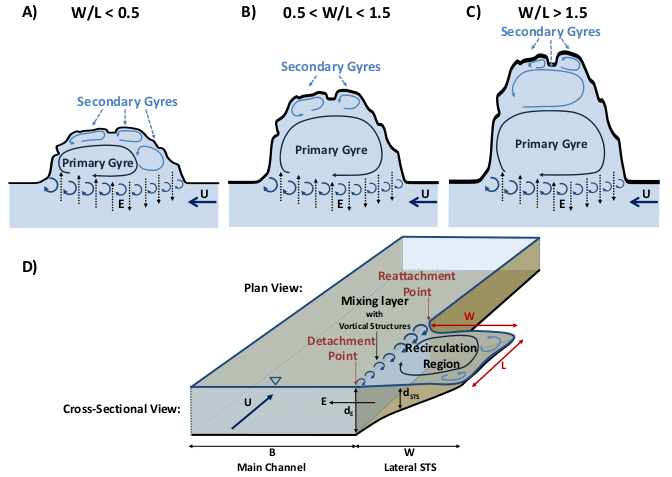
\includegraphics[width=0.9\linewidth]{../images/introduction/lateralCavitySchema.png}
\caption{Schema on the flow patterns of emergent lateral cavities \cite{jackson2013}}
\label{fig:lCavitySchema}
\end{figure}

\begin{figure}[!ht]
\centering
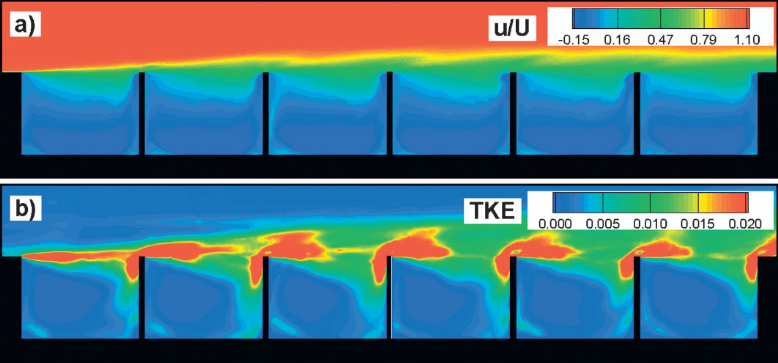
\includegraphics[width=0.9\linewidth]{../images/introduction/groyneStabilisation.png}
\caption{Time averaged quantities at $z/h=0.95$: a) streamwise velocity and b) TKE \cite{mcCoy2008}}
\label{fig:groyneStabilisation}
\end{figure}

The mass exchange between DZs and the main channel was vastly studied in field, experimental and numerical studies. Two different methods to estimate the velocity in which this exchange occurs are predominant: interface velocity measurements and tracer experiments.

As the effects of the exchange occur in a confined volume, \textcite{weitbrecht2001} proposed a model to account the exchanges in the interface between the zones. This method only requires geometrical parameters and the mean transversal velocity in the interface surface. Despite this planar method give a good approximation on the exchange velocity the effect of mass diffusivity and depth variation is neglected,  this further implies that systems slower circulations will have a larger impact of the estimated $k$, as the interface between the main channel and the cavity may remain with faster velocities. One can assume that this methodology works for conventional DZ, although it must be taken carefully for vegetated systems as the mixing layer alone may influence the result of $k$. 

Another approach on the mass exchange is through tracer experiments, that can be divided into washout and pulse procedures, that consists in the ejection of mass from the interior of the DZ and a pulse at the inlet of the channel, respectively.  Tracer methods treat the mass exchange tri-dimensionally as all the flow variables are considered. This approach gives a better understanding of the exchange in all conditions as it provides more information, for instance, the tracer methodology allows one to study the behaviour of mass in local regions of the volume or as a global volume. Furthermore, the coherent structures of the interface play a significant role in the transport of the tracer, given that the turbulence motion is transient, this method can capture the mass exchange rates over time and provide a better insight of the effect of those flow structures.

The advantage of the tracer method is the data richness that it provides, especially in numerical experiments. Some additional studies can be done to analyse other phenomena associated to mass, for instance, one can use a decay to estimate the amount of mass that is treated by plants or a settling velocity to preview sedimentation in the DZ. The only side effect of this method is the increased complexity to perform these experiments, be the difficulty in controlling the volume of water in the field or the calibration of the turbulent Schmidt number ($S_{ct}$) in numerical studies. 
\section{Ecology and Vegetation}
The presence of vegetation in river can also influence the hydrodynamics of the DZ and ,thus, the dispersion of solutes. Since the vegetation cover in rivers is dynamic, changing with seasonality and global climatic change, the dispersion of solutes in rivers is also dynamic. \cite{sukhodolova2006}, for example, studied the influence of the seasonality upon the longitudinal dispersion in a lowland river with vegetation. They observed that when vegetation is absent, the dead zones are represented predominantly by recirculation zones formed by flow separation on bank irregularities; in vegetative period, the dead zones are formed by blocking effect of vegetation occupying part of the river cross-section. These dead zones cause an increase of longitudinal dispersion, which means stronger lengthening of a solute cloud in the mainstream direction \cite{weitbrecht2004}.

The influence of vegetation in the mass exchange in lateral cavities was first studied in \textcite{xiang2019}, that will be discussed in this paragraph. In this paper, a single lateral cavity was studied with a varied vegetation density. The vegetation was represented as solid cylinders inside the cavity volume. The cavity was emergent with a single circulation, due to its $W/L=0.6$. The vegetation density ($a$) ranged from 0 to $6.27\permil$ and as it increased more drag was introduced into the flow resulting in a slower circulation inside the volume. The turbulent kinetic energy in the DZ gradually due to the blockage that impeded high energy vortexes from entering the volume. The effect on mass exchange occurred in two phases: first, there was a decay in the mean residence time due to the plant induced Karman vortex street and the plant blockage since the mixing rate from the vortex is greater than the blockage; in a second phase $a>3.96\permil$ the blockage was higher than the mixing what increases of mean residence time (Figure \ref{fig:xiang2019fig12}).
\begin{figure}[!ht]
\centering
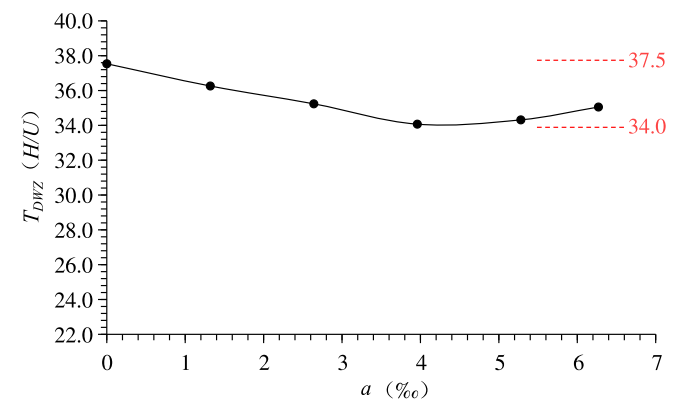
\includegraphics[width=0.8\linewidth]{../images/introduction/xiang2019fig12.png}
\caption{The variation of mean residence time ($T_{DWZ}$) with the increase of vegetation density ($a$) \cite{xiang2019}.}
\label{fig:xiang2019fig12}
\end{figure}

Although researchers have been studying the effect of groynes and vegetation on dispersion of solutes in rivers over the last decades (e.g. \textcite{sukhodolov2017,xiang2019,xiang2020}, there are still issues to that were not examined. For instance, in a vegetated groyne the vegetation levels were up to $15.7\permil$ \cite{sukhodolov2017}, a larger vegetation density range may contain other phenomena that could not appear in the previous studies. This hypothesis indicates that studying the variation of density until the vegetation resistance blocks the flow would cover all the possible ranges and thereby phenomena associated with this flow. Second, up to now the effects of the vegetation on the instantaneous fields were not investigated on lateral cavities. Third, the mass transfer at the main channel/dead zone was mainly studied using only the velocity at the interface, this leads to the opportunity of further describe the behaviour of mass inside the dead zone volume and how it affects the total exchange.

Furthermore, the study with vegetated cavities still could not identify a threshold for vegetation to be considered "dense" or "sparse" in cavities, and its understanding will allow researchers to identify flow modifications in the cavity (e.g., the suppression of recirculation gyres, the complete suppression of flow, the exchange coefficient asymptote, etc.).  For emergent vegetation patches in an open channel, \textcite{chen2012} characterised them as being “dense” or “sparse” according to flow blockage thresholds, in which the flow properties near the patch (e.g., flow adjustment length and the velocity exiting the patch) were distinct above and below the threshold. A similar approach can be done for vegetated cavities. 
\section{Objective and Research Questions}
In order to address this issues, the objective of this study is:

\textit{To describe the hydrodynamics and the mass exchange between vegetated dead waters and
the undisturbed section of the flow for different vegetation densities.}

The main hypothesis is that there is a threshold between dense and sparse vegetation in dead water. We also hypothesised that there is a threshold where the flow ceases inside the lateral cavity. 

Specific methodological objectives:
\begin{itemize}[noitemsep,topsep=0pt,align=left,itemindent=\parindent]
    \item The choice of the modelling technique;
    \item The choice of the modelling package (open and commercial software);
    \item The method to represent the vegetation drag.
\end{itemize}

\section{Dissertation Structure}
The dissertation was divided into six chapters. Following the Introduction, the first paper is presented where the methodology of the study of groyne fields is firstly introduced. Thirdly, the presented paper discussed the first approach to the study of lateral cavities. Fourthly, further development of the numerical model is presented, this implementation focused on the accessibility of the model by making use of open-source tools. Fifth, the main topic of this dissertation is introduced in the paper that describes the influence of the vegetation density in lateral cavities. Finally, the conclusive remarks about the flow in DZ and its mass exchange were presented.

